\chapter{Task 46: EU transportation network II}
\section{Task Description}
The aim of this task is to reconstruct the railway networks of European countries from the raw geographical data provided in the open database
\parencite[][ \textit{EuroGlobalMap}, $2019$ release]{euroglobalmap}. The requested output for each network is two files: one containing the edge list and one containing the node metadata \textit{[nodeLabel, latitude, longitude, country\_name, country\_ISO3]}.
\section{Data extraction}
The choice of what exactly the nodes of the network should represent is not specified (a possibility is to identify nodes with cities, but one could also opt for administrative district or even larger regions).
I decided to build networks where \textbf{nodes} correspond to \textbf{cities} where a railway station is present, and two nodes are connected through an \textbf{edge}  if they are \textbf{consecutive stops} of some rail. The accomplishment of this task was not straightforward. The best way I found involves first creating a preliminary network, where nodes do not have any specific physical significance, and, subsequently, extracting the desired network as a subset of it. \newline \noindent
I consulted \textit{EGM19\_DataSpecification.pdf, 
 Annex C - Definition of Features and Attributes} to understand what files I needed to look for in the database, Python library GeoPandas to open the shapefiles and NetworkX to create and manipulate graph objects. Station's data encoded in \textit{Point} objects containing the station's latitude and longitude, while railway data is encoded in \textit{LineString} objects, which are lists of points that connected together form a segmented line.
Besides, geometrical data comes with a number of attributes. These include :'ICC', the 2- character country IS03 code (es. IT, for Italy),  'NAMA1', the station name, and 'EXS', the existence category of the rail (e.g. abandoned, operational, under construction...).
\medskip \newline \noindent
As said already, in my method the desired networks are extracted as a subset of a preliminary network. 
The latter is built upon the data contained in file \textit{RailrdL.shp} with the following steps:
\newline \noindent
\begin{minipage}{0.5\textwidth}
\begin{enumerate}
    \item open the shapefile \textit{RailrdC.shp/.shx/.dbf} with Geopandas and extract relevant attributes
     \item initialize an empty graph with NetworkX
     \item iterate through the dataframe rows. For each LineString object, assign each of its point-like components to a node of the graph. Draw an edge between each pair of successive components.
\end{enumerate}
Figure [Fig: \ref{fig:raw}] shows what the resulting network looks like. At this stage, the nodes have no particular physical meaning: they are just the starting and ending points of the straight segments that make up the rail line.
\end{minipage}
\hfill
\begin{minipage}{0.48\textwidth}
    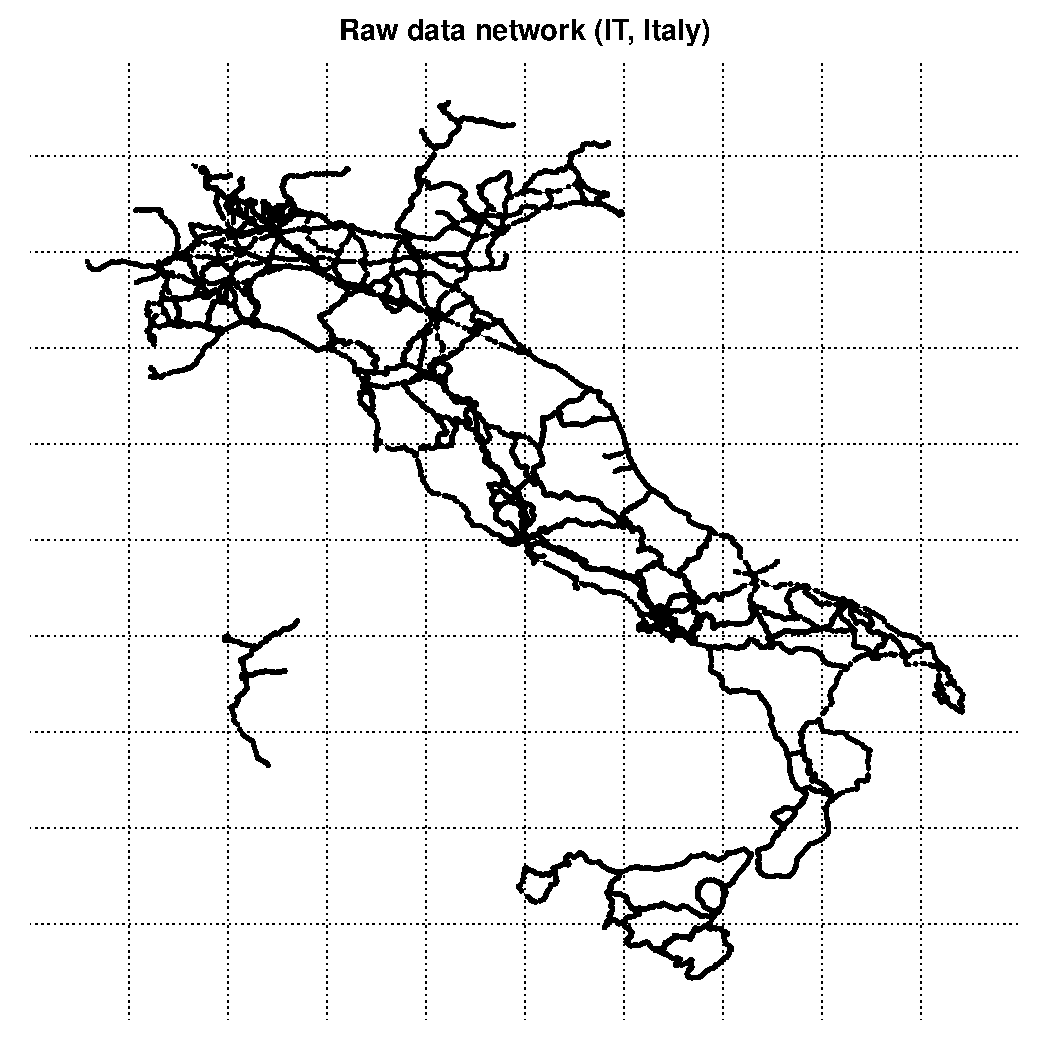
\includegraphics[width = \textwidth]{latex_source/images/railways/raw_networks/raw_IT_network.pdf}
    \captionof{figure}{}
    \label{fig:raw}
\end{minipage}
\bigskip \newline 
The following step consists in selecting only the nodes which corresponds to actual city stations, and rewire the links. To achieve this:
\begin{enumerate}
    \item city stations data is loaded from file \textit{RailrdC.shp/.shx/.dbf},
    \item \textit{Node labeling}: two new attributes are assigned to nodes of the preliminary network: "label" and "is\_near\_city". These fields are both "empty" by default.
    A loop checks if the preliminary network nodes' coordinates match any of the stations coordinates within a given threshold distance $d$. Nodes in the preliminary network are very dense, and in general more than one node will satisfy the threshold condition. The best match is assigned attribute "label = station\_name", while the others that also satisfy threshold are assigned "is\_near\_city = station\_name". 
    \item a new empty network is initialized and the nodes of the preliminary network with "label" $\neq$ "empty" (i.e. all the best matches) are added to it,
    \item \textit{Edge creation}: a maximum radius parameter $R$ is defined. The presence of an edge is checked only for the pair of nodes within distance $<2\,R$. The other pairs are assumed to not be connected: this introduces a possible error source but was necessary to obtain feasible computations.
    \item For each node pair in the new graph, the shortest paths between them in the \textit{old} graph is calculated. If a shortest path exists where all intermediate nodes have both fields "label" and "is\_near\_city" $\equiv$ "empty" (i. e. there exists a rail which connects the cities with no intermediate stops), these nodes are connected with an edge in the new graph.
\end{enumerate}
Notice that two threshold parameters $d$ and $R$ where added in this procedure. They were tuned by trial and error, and depended upon the country considered. The introduction of the auxiliary attribute "is\_near\_city" may seem unnecessary, but was motivated by data inspection [see Appendix, figure \ref{fig:bifurcation}]. In fact, rail bifurcations often start slightly before or after entering a city station. In reality, the train must pass through the city station even if it takes the bifurcation. Without the "is\_near\_city" field, the final network contained more edges than it should. Results for Italy are shown in [Figure: \ref{fig:rail_results}], while all other networks visualizations are in GitHub repository.
\begin{figure}[H]
\centering
    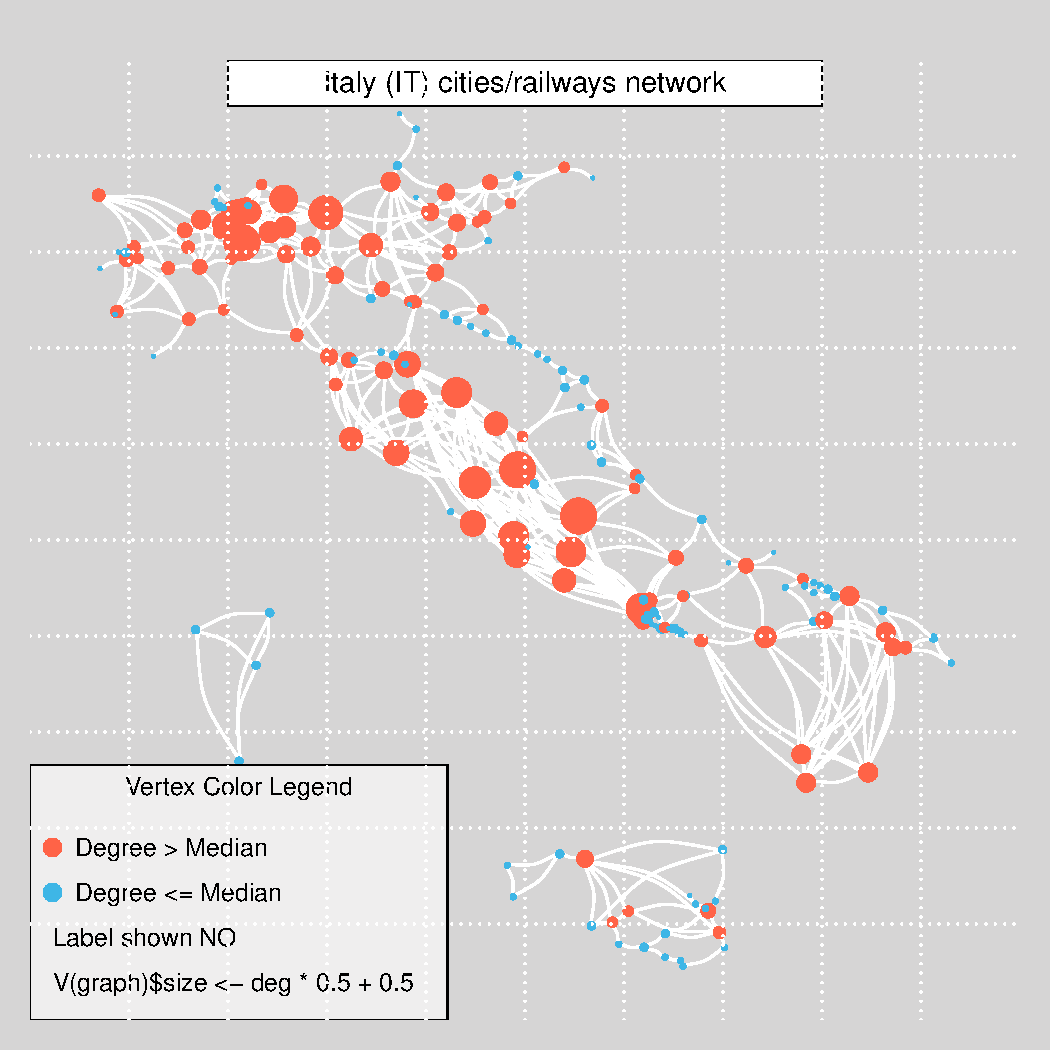
\includegraphics[width = 0.7\textwidth]{latex_source/images/railways/city_networks/IT_network.pdf}
\begin{subfigure}{}
    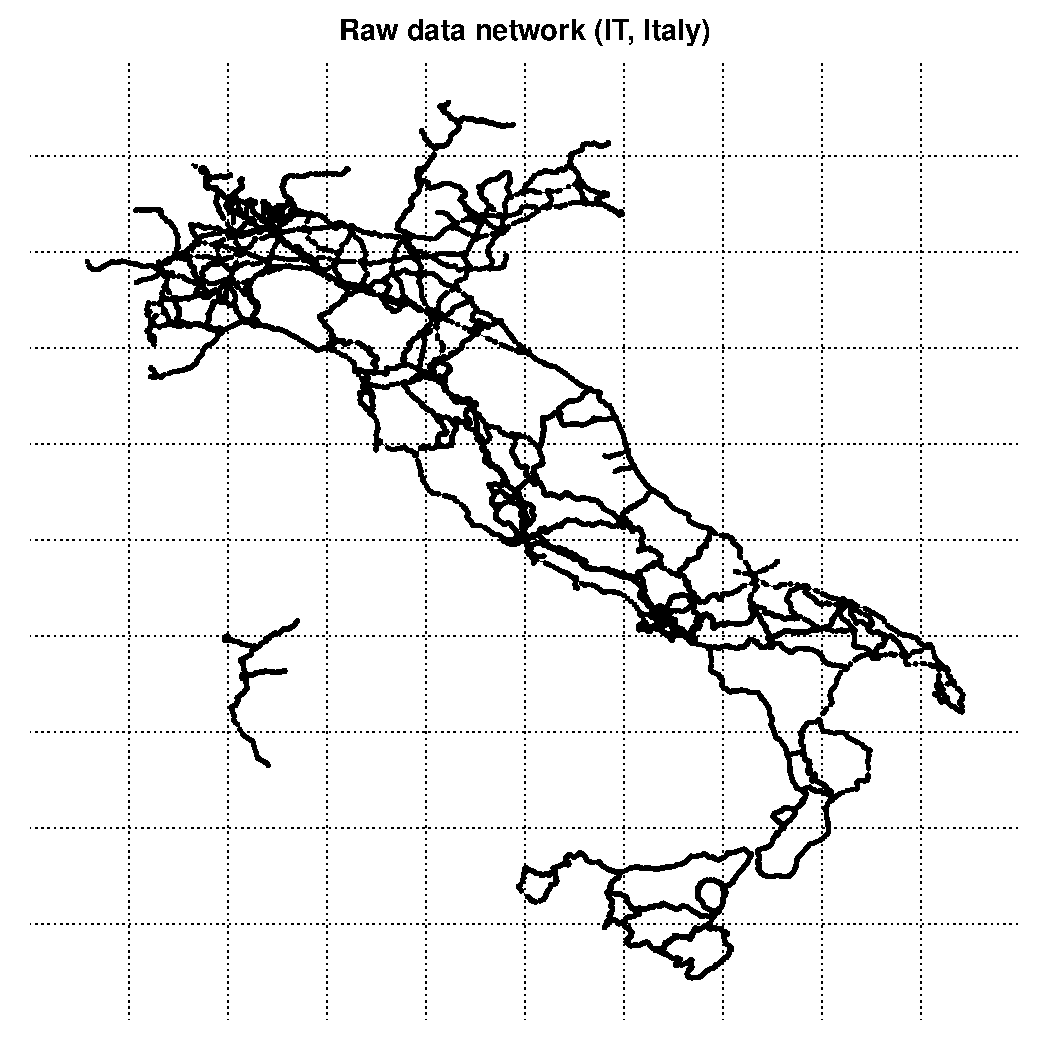
\includegraphics[width = 0.3\textwidth]{latex_source/images/railways/raw_networks/raw_IT_network.pdf}
\end{subfigure}
\begin{subfigure}{}
    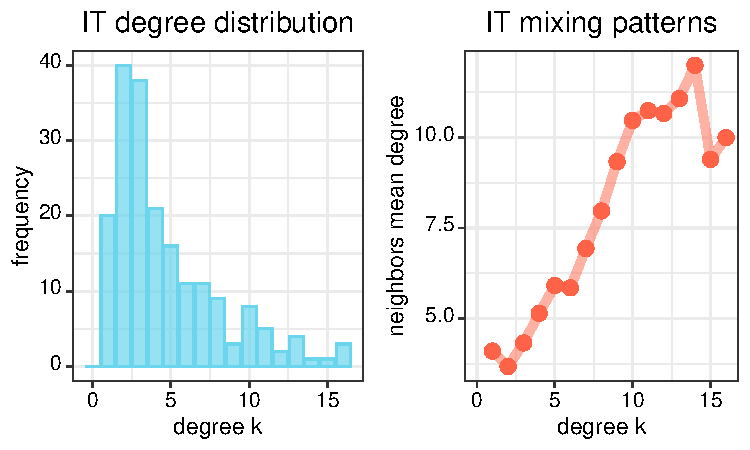
\includegraphics[width = 0.6\textwidth]{latex_source/images/railways/city_network_analysis/IT_analysis.pdf}
\end{subfigure}
\caption{IT (Italy) cities/ railways networks. Notice for instance the high density of edges in the center-left zone of the graph: it is a consequence of the fact that the stations "Roma Termini" and "Roma Tiburtina" are missing from file "RailrdC.shp" ! Many stations result directedly connected where in reality they are not because Rome stations are in between.}
\label{fig:rail_results}
\end{figure}
\newpage
\section*{Appendix}
\addcontentsline{toc}{section}{Appendix}
\subsection*{Supplementary figures}
\begin{figure}[H]
    \centering
    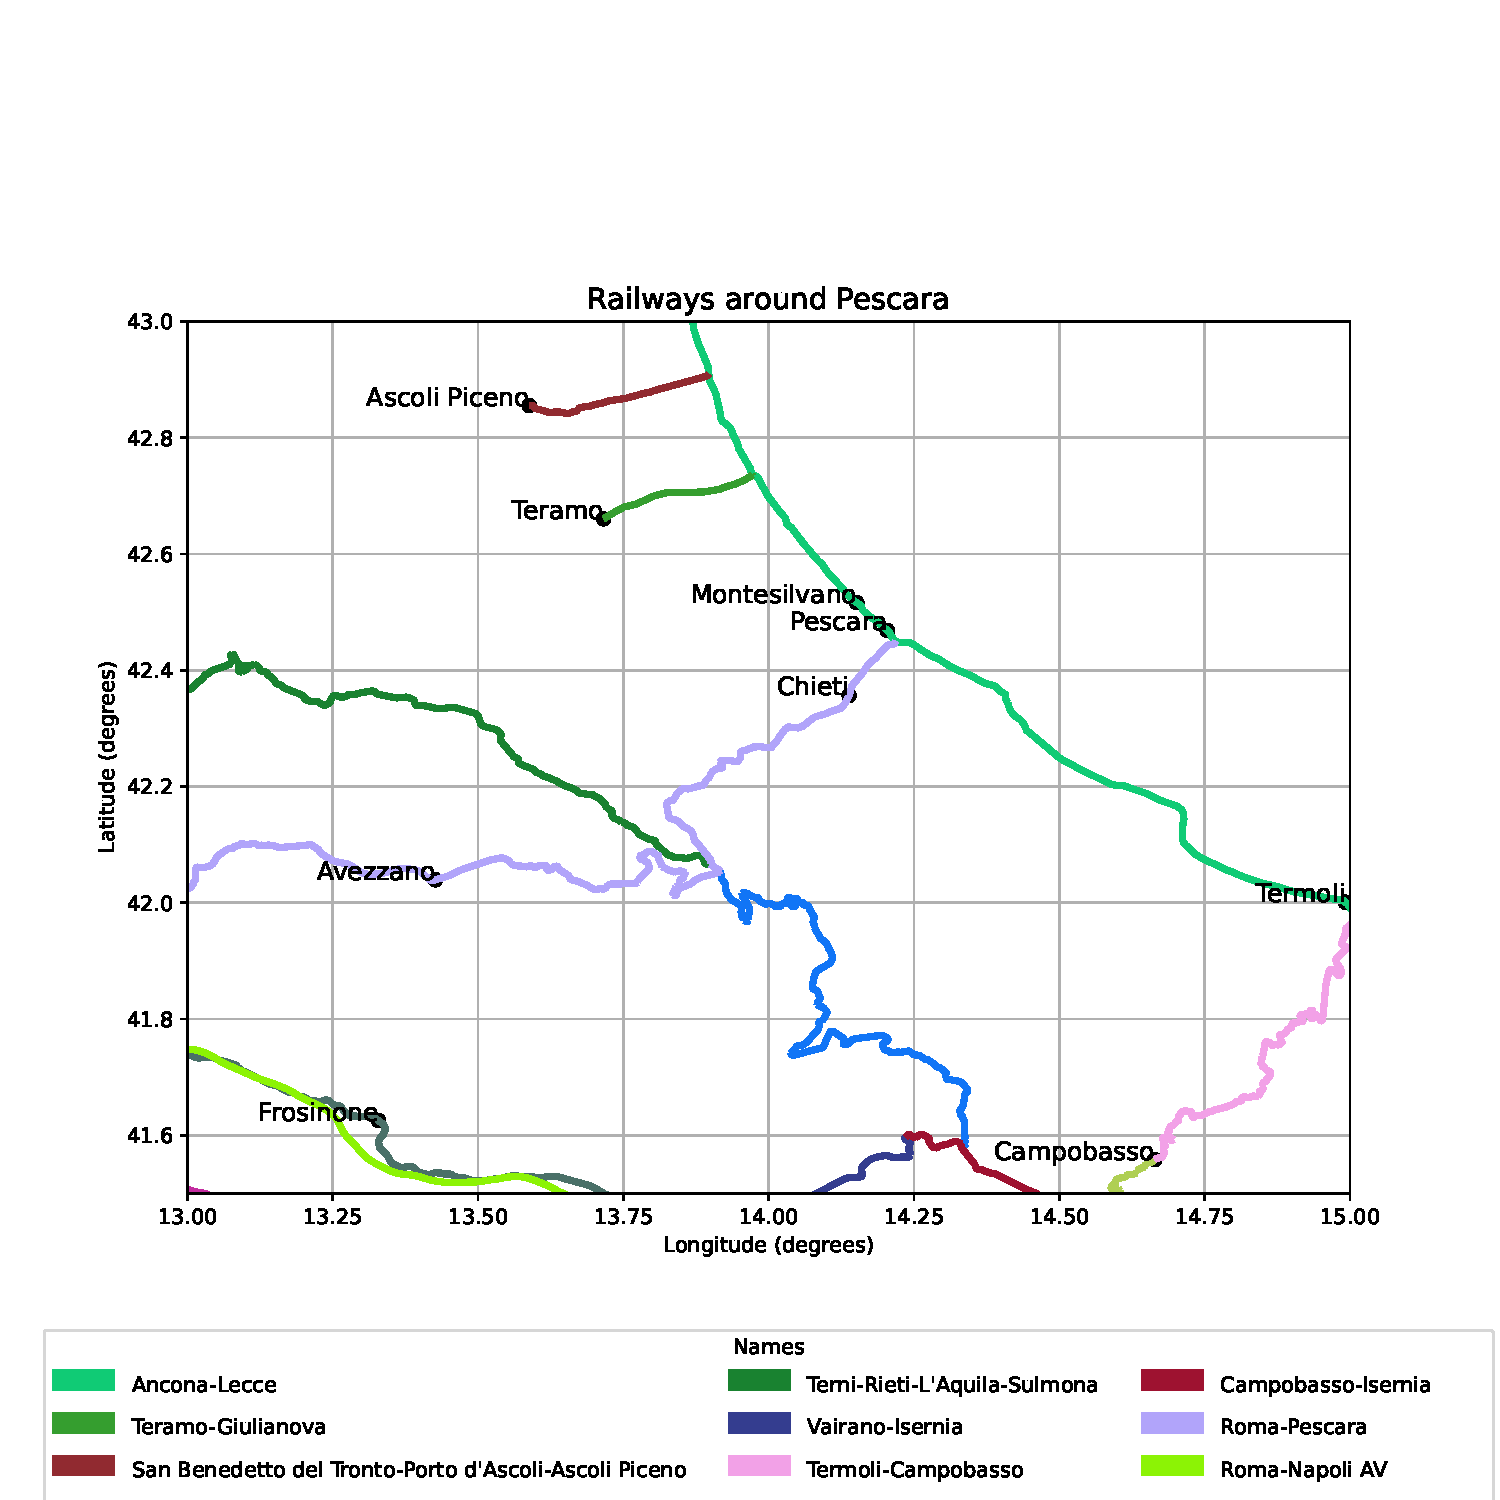
\includegraphics[width= \textwidth]{latex_source/images/railways/pescara_area.pdf}
    \caption{An example to justify the need for the "is near city" check: the rail bifurcation "Roma - Pescara" joins the "Ancora - Lecce" rail just before entering Pescara from south. Without the check implementation, edge "Termoli-Chieti" is created whereas in reality it does not exist: a train heading to Chieti must first stop in Pescara. }
    \label{fig:pescara_area}
\end{figure}
